% ============================================================
%  Chapter 1: Introduction and Motivation
%  Enhanced to include OpenFaaS, Two-Phase RL, and structured TikZ
% ============================================================
\chapter{Introduction and Motivation}
\label{chap:intro}

% ──────────────────────────────────────────────────────────────────────────────
\section{Background}
% ──────────────────────────────────────────────────────────────────────────────

The modern computing landscape has been profoundly influenced by the proliferation of 
connected devices. Sensors embedded in industrial systems, home automation networks, 
smart city infrastructures, and healthcare monitoring equipment generate continuous 
data streams. The analytical processing of these streams can yield valuable real-time 
insights \cite{hendrickson2020serverless}. Traditional cloud infrastructures, while 
computationally powerful, require explicit cluster provisioning and continuous management. 
This static rigidity proves highly inefficient for bursty Internet of Things (IoT) workloads, 
where traffic volumes fluctuate sharply and unpredictably \cite{shahrad2020serverless}.

To address the limitations of static provisioning, \textbf{serverless computing} abstracts 
server management by allocating resources dynamically in response to demand, charging 
only for the exact compute time consumed (often referred to as \textit{scale-to-zero}). 
Major cloud providers---including Amazon Web Services (AWS Lambda, EMR Serverless), 
Google Cloud (Cloud Functions, Dataproc Serverless), and Microsoft Azure---have introduced 
platforms that extend beyond simple function execution to include massive distributed 
analytics engines such as Apache Spark.

Apache Spark has long been the dominant framework for large-scale data analytics. In its 
\textbf{Structured Streaming} mode, Spark can handle continuous streams of events with 
micro-batch or near-real-time semantics. Integrating Spark with a serverless backend provides 
the theoretical promise of infinite scalability and cost efficiency. However, in practice, 
deciding \textit{when} and \textit{how much} to scale in real-time introduces critical 
new challenges in autonomous resource optimization \cite{werner2024reference, pu2019shuffling}.

% ──────────────────────────────────────────────────────────────────────────────
\section{Need for a Serverless Spark Framework}
% ──────────────────────────────────────────────────────────────────────────────

Conventional Spark streaming clusters require the manual, upfront configuration of 
logical parameters: the number of executors, their memory allocations, and core counts. 
Inefficient parameter choices lead directly to severe performance degradation. If provisioned 
too low, the cluster suffers from overwhelming backpressure and latency spikes, violating 
critical Service Level Agreements (SLAs). If provisioned too high, the cluster wastes expensive 
compute cycles sitting idle \cite{eismann2021serverless}. 

While serverless platforms abstract away the \textit{physical} infrastructure, the 
\textit{logical} configuration parameters still mathematically dictate performance. 
The dynamic, non-stationary nature of IoT workloads demands an intelligent, adaptive mechanism 
capable of adjusting these parameters in real time without human intervention 
\cite{shahrad2020serverless}. Specifically, there is a distinct need for a control plane 
that can shift its strategy autonomously---minimizing costs during quiet night hours, 
but preemptively scaling up to prevent latency spikes during intense data bursts.

% ──────────────────────────────────────────────────────────────────────────────
\section{Challenges in IoT Data Processing}
% ──────────────────────────────────────────────────────────────────────────────

\begin{figure}[H]
\centering
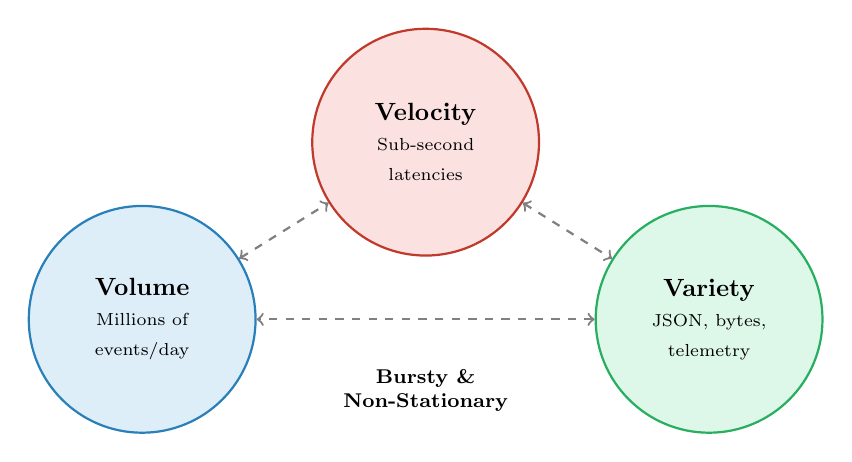
\begin{tikzpicture}[
    circlebox/.style={circle, draw=black, thick, minimum size=3.2cm, align=center},
    scale=0.9, transform shape
]

% Colors
\definecolor{voldraw}{RGB}{41,128,185}
\definecolor{volfill}{RGB}{214,234,248}

\definecolor{veldraw}{RGB}{192,57,43}
\definecolor{velfill}{RGB}{250,219,216}

\definecolor{vardraw}{RGB}{39,174,96}
\definecolor{varfill}{RGB}{213,245,227}

% Circles
\node[circlebox, draw=voldraw, fill=volfill, fill opacity=0.8, text opacity=1] (vol) at (0,0) 
    {\textbf{Volume} \\ \scriptsize Millions of \\ \scriptsize events/day};

\node[circlebox, draw=veldraw, fill=velfill, fill opacity=0.8, text opacity=1] (vel) at (4,2.5) 
    {\textbf{Velocity} \\ \scriptsize Sub-second \\ \scriptsize latencies};

\node[circlebox, draw=vardraw, fill=varfill, fill opacity=0.8, text opacity=1] (var) at (8,0) 
    {\textbf{Variety} \\ \scriptsize JSON, bytes, \\ \scriptsize telemetry};

% Intersecting text
\node[font=\footnotesize\bfseries, align=center] at (4, -1) {Bursty \& \\ Non-Stationary};

% Arrows showing interaction
\draw[<->, thick, dashed, gray] (vol) -- (vel);
\draw[<->, thick, dashed, gray] (vel) -- (var);
\draw[<->, thick, dashed, gray] (var) -- (vol);

\end{tikzpicture}
\caption{The ``3V'' challenges of IoT workloads. The intersection of these forces creates highly unpredictable, bursty traffic patterns that routinely break static scaling rules.}
\label{fig:3v_iot}
\end{figure}

IoT data differs from conventional batch data in three fundamental aspects defined by the ``3Vs'': \textbf{Volume}, \textbf{Velocity}, and \textbf{Variety} \cite{kjorveziroski2021iot}. Continuous, heterogeneous sensor streams impose stringent latency requirements, especially for critical real-time applications such as autonomous vehicle fleet monitoring or industrial safety feedback loops \cite{chen2021edge}. 

When building a serverless processor for these demands, four massive challenges emerge:
\begin{enumerate}
  \item \textbf{The Scale-to-Zero Cold Start Problem:} Modern serverless functions shut down when idle to save money. When a sudden burst of IoT traffic arrives, booting new containers takes 45--60 seconds (the ``cold start''), during which real-time data is delayed or dropped en masse.
  \item \textbf{Reactive Blindness:} Standard auto-scalers (like Kubernetes HPA) are strictly reactive. They only scale \textit{after} CPU thresholds are broken, which is already too late to prevent an SLA violation during a tsunami of sensor data.
  \item \textbf{Cost vs.\ Performance Tug-of-War:} Maximizing throughput requires over-provisioning executors, which destroys cost efficiency. Minimizing cost requires running edge-case minimums, which ruins latency.
  \item \textbf{The Static Policy Limitation:} A system cannot use the same scaling strategy at 3:00 AM (when traffic is minimal and cost should be prioritized) as it does at 9:00 AM (when traffic bursts require aggressive latency protections).
\end{enumerate}

% ──────────────────────────────────────────────────────────────────────────────
\section{Motivation}
% ──────────────────────────────────────────────────────────────────────────────

Manual tuning and threshold-based heuristics fail completely when forced to cope with the unpredictable, non-stationary nature of IoT traffic. Hand-coded rules (e.g., \textit{``if CPU > 80\%, add 2 executors''}) respond too slowly and lead to severe oscillating feedback loops. Standard predictive models trained offline often generalize poorly when seasonal workload patterns shift \cite{nestorov2024dexter}. 

Deep Reinforcement Learning (DRL) offers a compelling and radically different alternative. By treating cluster configuration as a continuous, sequential Markov Decision Process (MDP), an RL agent can learn highly complex resource-allocation strategies directly through trial, error, and reward interaction with the environment \cite{zhou2024deep}. Specifically, algorithms like **Proximal Policy Optimization (PPO)** enable stable, continuous adaptation \cite{schulman2017ppo}. 

Furthermore, simply embedding an RL script inside a Spark Driver is structurally insufficient. To achieve true cloud-native cost efficiency, the intelligence engine itself must be decoupled from the data engine. This motivates the need to deploy the RL ``brain'' strictly as a serverless function (via platforms like OpenFaaS), allowing the control plane to physically scale to zero when not in use.

% ──────────────────────────────────────────────────────────────────────────────
\section{Objectives}
% ──────────────────────────────────────────────────────────────────────────────

The overarching goal of this research is to build an autonomous, latency-aware, and highly cost-efficient IoT data processing pipeline. To achieve this, the project establishes the following specific objectives:

\begin{enumerate}
  \item \textbf{Modular Pipeline Design:} To design and construct a fully containerised, 5-layer serverless architecture tailored to real-time IoT ingestion and edge-to-cloud processing using MQTT, Kafka, and Spark \cite{werner2024reference}.
  
  \item \textbf{Two-Phase RL Optimization Engine:} To develop a novel Hierarchical Reinforcement Learning controller that fuses a TD3 Meta-Controller (for strategic, long-term reward shaping) with a PPO Resource Agent (for tactical, immediate scaling actions) to dynamically balance latency, throughput, and cost.
  
  \item \textbf{Serverless Function Decoupling:} To package and deploy the trained RL inference engine using OpenFaaS, establishing an HTTP-driven, scale-to-zero control plane that is fully decoupled from the JVM-heavy Spark executors.
  
  \item \textbf{Cold-Start Mitigation:} To implement a mathematical Pattern Feature Extractor at the IoT edge capable of generating probabilistic burst metrics, allowing the RL agent to \texttt{PRE\_WARM} Spark containers entirely avoiding serverless cold-start penalties.
  
  \item \textbf{Empirical Evaluation:} To rigorously benchmark the proposed architecture against existing heuristic and regression-based Horizontal Pod Autoscaler (HPA) platforms \cite{nestorov2024dexter} across diverse, 24-hour non-stationary workload scenarios.
\end{enumerate}

% ──────────────────────────────────────────────────────────────────────────────
\section{Scope of Work}
% ──────────────────────────────────────────────────────────────────────────────

This work focuses on the integration of Apache Spark Structured Streaming with a containerized event-driven architecture. The scope extends deeply into logical resource optimization modeling (dynamic executor provisioning, variable memory allocation, and predictive pre-warming).

The research \textit{includes} the offline simulation of cluster dynamics for RL training, the deployment of OpenFaaS as a serverless gateway, and the construction of synthetic, multi-domain edge IoT generators. 

The scope \textit{excludes} low-level Linux kernel network scheduling, physical hardware-specific CPU pinning, and custom modifications to the internal Apache Spark DAG scheduler \cite{pu2019shuffling}. The validation is conducted via Dockerized environments modeling cloud behaviors, preparing the system for lift-and-shift deployment to commercial environments like AWS EMR.

% ──────────────────────────────────────────────────────────────────────────────
\section{Expected Outcomes and Thesis Structure}
% ──────────────────────────────────────────────────────────────────────────────

The proposed framework is expected to deliver state-of-the-art performance in real-time, burst-heavy data analytics. The expected measurable outcomes include:
\begin{itemize}
  \item \textbf{Elimination of SLA Violations} through edge-driven cold-start pre-warming.
  \item \textbf{Drastic reductions in idle computing costs} via OpenFaaS scale-to-zero decoupling compared to always-on traditional models.
  \item \textbf{Superior multi-objective adaptability} enabled by the TD3 Meta-Controller seamlessly shifting strategy contexts without human intervention.
\end{itemize}

\subsection{Organization of the Thesis}

The remainder of this thesis is structured as follows:
\begin{itemize}
    \item \textbf{Chapter 2 (Literature Review):} Explores existing work in serverless analytics, static heuristics, and recent applications of RL in cloud computing.
    \item \textbf{Chapter 3 (System Architecture):} Details the design of the 5-layer IoT data pipeline, tracing the data flow from MQTT edge generators through Kafka and down to Spark.
    \item \textbf{Chapter 4 (RL-Based Resource Optimizer):} Covers the theoretical foundation, MDP formulation, and implementation of the Phase-1 PPO tactical agent.
    \item \textbf{Chapter 5 (Hierarchical RL and OpenFaaS):} Introduces the Phase-2 TD3 Meta-Controller and the architectural deployment of the RL orchestrator as an OpenFaaS serverless function.
    \item \textbf{Chapter 6 (Results and Discussion):} Presents the full empirical evaluation, showcasing cost, latency, and SLA compliance against competitive baselines using 24-hour trace simulations.
    \item \textbf{Chapter 7 (Conclusion and Future Work):} Summarizes the core intellectual contributions and outlines a roadmap toward multi-agent and sustainably-aware scaling.
\end{itemize}
